\documentclass{article}
\usepackage{tikz}
\usetikzlibrary{shapes,snakes}
\usepackage{verbatim}

\begin{comment}
:Title: Node shapes
:Tags: Basics, Nodes and shapes, Matrix, PGF 1.18

An overview of predefined node shapes. Note that only the ``rectangle`` and
``circle`` shapes are loaded by default. To use other shapes, load the
``shape`` library. The ``regular polygon`` and ``star`` shapes are only available for PGF >= v 1.18.

\end{comment}



\begin{document}

\pagestyle{empty}

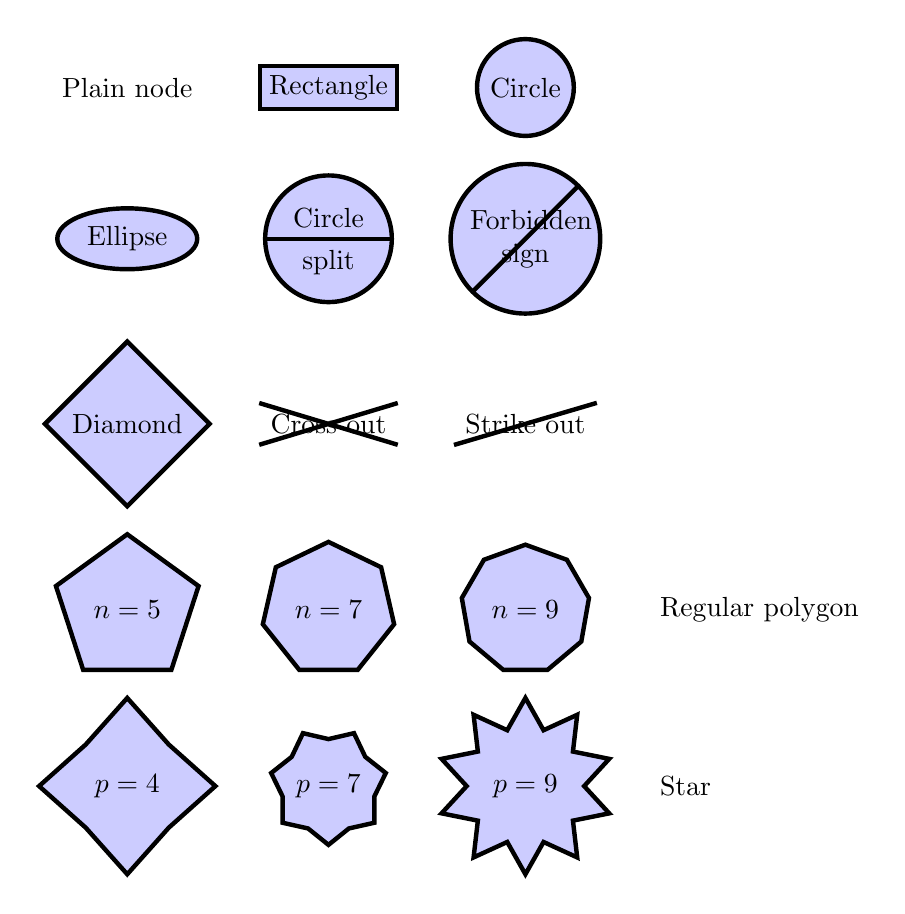
\begin{tikzpicture}[scale=2]
    \tikzstyle{ann} = [draw=none,fill=none,right]
    \matrix[nodes={draw, ultra thick, fill=blue!20},
        row sep=0.3cm,column sep=0.5cm] {
    \node[draw=none,fill=none] {Plain node}; &
    \node[rectangle] {Rectangle}; &
    \node[circle] {Circle};\\
    \node[ellipse] {Ellipse};&
    \node[circle split] {Circle \nodepart{lower} split};&
    \node[forbidden sign,text width=4em, text centered]
                    {Forbidden sign};\\
    \node[diamond] {Diamond};&
    \node[cross out] {Cross out};&
    \node[strike out] {Strike out};\\
    \node[regular polygon,regular polygon sides=5] {$n=5$};&
    \node[regular polygon,regular polygon sides=7] {$n=7$};&
    \node[regular polygon,regular polygon sides=9] {$n=9$};&
    \node[ann]{Regular polygon};\\
    \node[star,star points=4] {$p=4$};&
    \node[star,star points=7,star point ratio=0.8] {$p=7$};&
    \node[star,star points=10] {$p=9$};&
    \node[ann]{Star};\\
    };
\end{tikzpicture}


\end{document}

